\appendix

\section{Anhang: Erg�nzende Projektvereinbarungen}

\subsection{Projektorganisation}

\begin{table}[!h]
 \begin{center}
 \begin{tabular}{|l|l|}
 \hline
 Projektteam      &  M. Bigler (\href{mailto:biglm2@hta-bi.bfh.ch}{biglm2@hta-bi.bfh.ch}) \\
                  &  S. R�ss (\href{mailto:rasss@hta-bi.bfh.ch}{rasss@hta-bi.bfh.ch})     \\
                  &  L. Zbinden (\href{mailto:zbinl@hta-bi.bfh.ch}{zbinl@hta-bi.bfh.ch})  \\
 \hline
 Projektleiter    &  S. R�ss (\href{mailto:rasss@hta-bi.bfh.ch}{rasss@hta-bi.bfh.ch}) \\
 \hline
 Projektbetreuer  &  J.-P. Dubois (\href{mailto:doj@hta-bi.bfh.ch}{doj@hta-bi.bfh.ch}) \\
                  &  C. Fuhrer (\href{frc@hta-bi.bfh.ch}{frc@hta-bi.bfh.ch}) \\
 \hline
 PM Couch         &  F. Helbling (\href{frank.helbling@helbling-consulting.ch}{frank.helbling@helbling-consulting.ch}) \\
 \hline
 \end{tabular}
 \end{center}
 \caption{Projektorganisation}
 \label{Projektorganisations Tabelle}
\end{table}

\begin{figure}[h]
  \begin{center}
    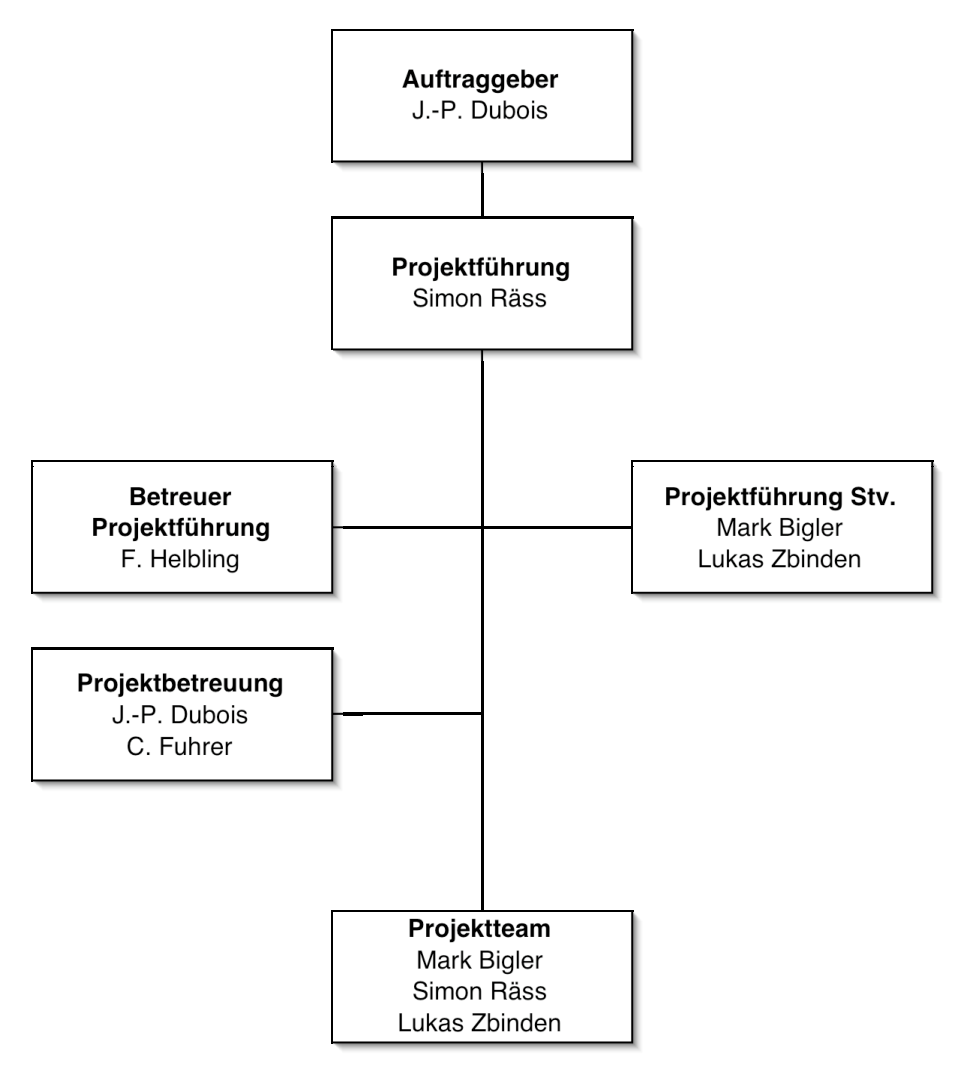
\includegraphics[width=10cm,height=9.2cm]{../../images/organigramm.eps}
  \end{center}
  \caption{Projektorganisation}
  \label{Projektorganisation}
\end{figure}


\subsection{Projektplanung}
Die genaue Projektplanung kann dem Projektplan entnomen werden.
\begin{table}[!h]
 \begin{center}
 \begin{tabular}{|l|l|}
  \hline
  Anfang der Semesterarbeit       &    21.02.2005 \\
  \hline
  Beginn der Initialiserungsphase &    21.02.2005 \\
  \hline
  Ende der Semesterarbeit         &    24.07.2005 \\
  \hline
 \end{tabular}
 \end{center}
 \caption{Projektplanung}
 \label{Projektplanung}
\end{table}

\subsection{Qualit�tssicherung}
F�r alle kritischen Stellen der Implementation m�ssen Unit Tests bestehen. F�r das Testen des Synchronisationsalgorithmus soll ein Testframework implementiert werden. Dieses soll es erm�glichen auch komplexe zeitliche Abfolgen zu definieren und wiederholt ablaufen zu lassen. Damit k�nnen pr�zise Testf�lle erstellt werden, die automatisiert und wiederholt ausgef�hrt werden k�nnen.

\subsection{Konfigurationsmanagement}
Es werden s�mtliche Dokumente des Projektmanagements, s�mtlicher Quellcode, die Inhalte der Website und die f�r die Erstellung des Programms ben�tigten externen Bibliotheken werden unter das Konfigurationsmanagement gestellt.

Die Projektdokumentation und Produktdokumentationen werden mit einer Versionskontrolle versehen. Die Dokumente k�nnen dabei die in der Tabelle \ref{Versionsnummern} angegebenen Zust�nde annehmen.

\begin{table}[!h]
 \begin{center}
 \begin{tabular}{|l|l|}
 \hline
 \headercol{0.6in}{Version}   &  
 \headercol{3in}{Bezeichnung} \\
 \hline
 0.1 - 0.99  &  Entwurfsversionen \\
 \hline
 1.0         &  erste Release Version \\
 \hline
 1.1         &  allf�llige �berarbeitete Versionen \\
 \hline
 \end{tabular}
 \end{center}
 \caption{Versionsnummern}
 \label{Versionsnummern}
\end{table}

F�r das Konfigurationsmanagement wird unser eigens installiertes Subversion Repository verwendet. Das entsprechende Repository ist unter \href{http://ace.iserver.ch:81/repos/ace/}{http://ace.iserver.ch:81/repos/ace/} erreichbar. Aus der commit Nachricht soll erkenntlich sein, wenn die Versionsnummer des Dokumentes erh�ht wurde. 


